\documentclass[tikz,border=1pt]{standalone}
\usepackage{stix}
\begin{document}
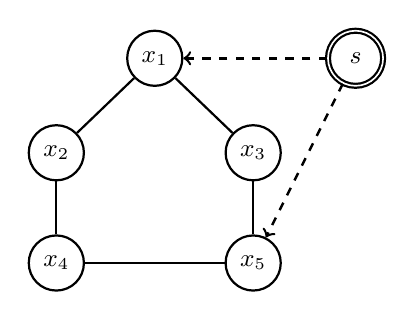
\begin{tikzpicture}[
		follower/.style={circle, draw, thick, minimum size=7mm, inner sep=0pt, font=\small},
		leader/.style={circle, draw, double, thick, minimum size=7mm, inner sep=0pt, font=\small},
		link/.style={line width=0.8pt},
		pin/.style={->, dashed, line width=0.9pt}
		]
		\node[leader] (s) at (2.55,1.55) {$s$};
		\node[follower] (x1) at (0,1.55) {$x_1$};
		\node[follower] (x2) at (-1.25,0.35) {$x_2$};
		\node[follower] (x3) at (1.25,0.35) {$x_3$};
		\node[follower] (x4) at (-1.25,-1.05) {$x_4$};
		\node[follower] (x5) at (1.25,-1.05) {$x_5$};
		\draw[link] (x1) -- (x2);
		\draw[link] (x1) -- (x3);
		\draw[link] (x2) -- (x4);
		\draw[link] (x3) -- (x5);
		\draw[link] (x4) -- (x5);
		\draw[pin] (s) -- (x1);
		\draw[pin] (s) -- (x5);
	\end{tikzpicture}
\end{document}
